% SPDX-License-Identifier: CC-BY-4.0
% Copyright (c) 2026 Alexander S. Donahue
\documentclass[11pt,letterpaper]{amsart}

\usepackage[margin=0.95in]{geometry}
\usepackage{amsmath,amssymb,amsthm,mathtools}
\usepackage{booktabs,array,multirow}
\usepackage{graphicx}
\usepackage{xcolor}
\usepackage{enumitem}
\usepackage{microtype}
\usepackage[hidelinks,pdfauthor={Alexander S. Donahue},pdftitle={Koszul-Veronese Byzantine Private Information Retrieval, MLWE Reduction Tightness, and Machine-Checked Complexity-Barrier Bridges}]{hyperref}

\theoremstyle{plain}
\newtheorem{theorem}{Theorem}[section]
\newtheorem{lemma}[theorem]{Lemma}
\newtheorem{proposition}[theorem]{Proposition}
\newtheorem{corollary}[theorem]{Corollary}

\theoremstyle{definition}
\newtheorem{definition}[theorem]{Definition}
\newtheorem{remark}[theorem]{Remark}
\newtheorem{example}[theorem]{Example}

\newcommand{\F}{\mathbb{F}}
\newcommand{\Z}{\mathbb{Z}}
\newcommand{\Q}{\mathbb{Q}}
\newcommand{\R}{\mathbb{R}}
\newcommand{\PP}{\mathbb{P}}
\newcommand{\GRS}{\mathrm{GRS}}
\newcommand{\CBD}{\mathrm{CBD}}
\newcommand{\Var}{\mathrm{Var}}
\newcommand{\Cov}{\mathrm{Cov}}
\newcommand{\rank}{\mathrm{rank}}
\newcommand{\spn}{\mathrm{span}}
\newcommand{\aff}{\mathrm{Aff}}

\title[Koszul--Veronese Byzantine PIR, MLWE Tightness, and Triad Barriers]{Koszul--Veronese Byzantine Private Information Retrieval,\\MLWE Reduction Tightness, and Machine-Checked\\Complexity-Barrier Bridges}

\author{Alexander S. Donahue}
\address{Independent Researcher, Spokane, WA, USA}
\email{0\_0@0thernes.art}
\urladdr{https://orcid.org/0009-0006-8168-9648}

\date{November 25, 2026 (Research Preprint, v1.0.0; not externally peer-reviewed)}
\subjclass[2020]{94A60, 94B05, 68Q15, 81P68, 03B35}
\keywords{Private information retrieval, Byzantine servers, Koszul--Veronese rank, Shannon--Ingleton barrier, Module-LWE, FIPS 203 ML-KEM, R\'enyi divergence, Quantum Geometric Tensor, Algebrization, Lean 4 formal verification}

\begin{document}

\begin{abstract}
We present fourteen zero-Mathlib Lean 4.35.0 machine-checked theorems (\texttt{T1a}--\texttt{T3d}) spanning three connected open frontiers: coded, colluding, robust, and Byzantine private information retrieval (PIR), post-quantum Module-LWE (MLWE) reduction tightness, and complexity-theoretic barriers around $\mathrm{P} \neq \mathrm{NP}$.
\textbf{Pillar I (Coded/Byzantine PIR):} We resolve the open Schur-product syzygy rank problem of Sun, Tao, Xu, and Zhang (\texttt{arXiv:2603.10769}) via a shifted-difference Koszul--Veronese identity proving $\lambda^\star(T,T',K) = \min\bigl(N\binom{T-1}{T'-1},\, K\binom{T}{T'},\, (K+T-T')\binom{T-1}{T'-1}\bigr)$. This collapses the universal $K \leftrightarrow T$ symmetric two-file rate to $R^{\mathrm{Koszul}} = E^2(E-1)/[(N-U)(E^2+(K+T-2)E-KT)]$ ($E := N - U - 2B$), strictly dominating the linear full-support-rank capacity of Sun and Zhang (\texttt{arXiv:2610.37412}) by exact numerator excess $(K-1)(T-1)E^2 > 0$ for all $K,T \ge 2$ (single-file and $P$-out-of-$M$ multi-file) and improving Example~VII.A of \texttt{arXiv:2603.10769} from $4/7$ to $10/17$. Using exterior-power subspaces $V_n = u_n \wedge \Lambda^{K-1}(\F_q^E)$ with single-orbit flag privacy, we construct zero-error schemes that: (i)~settle the exact linear capacity of $U$-$B$-MDS-$T$PIR for $(M=2, K=2, T=2)$ across all $E \ge 4$ (kernel-certified over $\F_{11}$ at rate $2/5 > 8/21$ for $N=6, B=1$); (ii)~achieve the \emph{exact unrestricted} (non-linear included) capacity at $E = K + 1$ for all $K \ge 2$, breaking the $E \ge KT$ feasibility barrier of \texttt{arXiv:2610.37412}; and (iii)~turn the $\epsilon$-error $T = 3$ schemes of \texttt{arXiv:2603.10769} into zero-error schemes, including $(N=6,K=3,T=3,B=0)$ at $10/17$ and Byzantine $(N=8,K=3,T=3,B=1)$ at $15/34$. Conversely, we construct and kernel-certify a 330-orbit pure-integer unconditioned 12-variable polymatroid $h_{\mathrm{uncond}}$ (scale~128) satisfying all 270{,}336 elemental Shannon inequalities, all 99 PIR equalities (including all 89 full $T=2$ privacy equalities), all 1{,}485 singleton Ingletons, and all 3{,}814{,}209 retrieval-subsystem Ingletons at rate $8/13 > 3/5 = C_{\mathrm{lin}}(2,4,2,2)$, paired with a field-universal projective $\PP^3$ impossibility theorem explaining why linear schemes collapse to $3/5$.
\textbf{Pillar II (MLWE Tightness):} We formally refute determinant-ideal module-SVP attacks (\texttt{arXiv:2604.15858}) over arbitrary commutative rings ($\det(B) = q^m$, independent of the MLWE secret), give a ring-universal algebraic proof of the Step-9 anti-periodic DFT cancellation ($\hat{f}(2k) \equiv 0$) in Chen (ePrint~2024/555), certify to 60-digit precision a $4.96\times$ R\'enyi-2 reduction-tightness cliff in NIST FIPS~203 ML-KEM from $\CBD_3$ (7.63~bits) to $\CBD_2$ (28.38~bits at ML-KEM-768; 37.84~bits at ML-KEM-1024), and establish a Quantum Geometric Tensor identity $\Omega_{\theta\sigma} = \Cov(X, (X-e_0)^2/\sigma^3)$ detecting shifted-LWE noise bias.
\textbf{Pillar III (Complexity Triad):} We formalize multilinear extension global uniqueness over any field (the algebraic core of Algebrization) alongside formal bridges linking LWE PRFs to Natural Proofs, $B$-Byzantine PIR to locally decodable code distance $d_{\min} \ge 2B+1$, and MLWE single-server PIR's sharp rounding margin $|e| \le 831$ to multi-server zero-noise PIR. \emph{We explicitly affirm that $\mathrm{P} \neq \mathrm{NP}$, non-linear $C(2,4,2,2) \in [3/5, 8/13]$, general $M \ge 3$ non-LFSR PIR capacity, and worst-case quantum MLWE lower bounds remain completely open.}
\end{abstract}

\maketitle

\section{Introduction and Claims Ledger}
\label{sec:intro}

Three long-standing open problems sit at the intersection of information-theoretic privacy, post-quantum cryptography, and computational complexity:
\begin{enumerate}[leftmargin=1.8em]
  \item \textbf{Coded, Colluding, Robust, and Byzantine PIR (\texttt{CS-053}):} Determining the exact download capacity of $U$-unresponsive, $B$-Byzantine, $T$-colluding Private Information Retrieval from an $(N, K)$-MDS coded storage system storing $M$ files~\cite{Chor1998,BanawanUlukus2018,FreijHollanti2017,SunJafar2017,Holzbaur2021,SunTaoXuZhang2026,SunZhang2026}.
  \item \textbf{Post-Quantum MLWE Reduction Tightness (\texttt{CS-026}):} Quantifying exact hardness and concrete reduction losses for Module-LWE as standardized in NIST FIPS~203 ML-KEM~\cite{Regev2009,LangloisStehle2015,Bai2018,NISTFIPS203}, and rigorously auditing proposed cryptanalytic attacks~\cite{Chen2024,Luo2026}.
  \item \textbf{Complexity-Theoretic Barriers Around $\mathrm{P} \neq \mathrm{NP}$ (\texttt{CS-001}) and Locally Decodable Codes (\texttt{CS-051}):} Mapping how cryptographic hardness and local decoding interact with Relativization~\cite{BakerGillSolovay1975}, Natural Proofs~\cite{RazborovRudich1997}, and Algebrization~\cite{AaronsonWigderson2009}.
\end{enumerate}

Rather than making speculative or unverified claims on open conjectures, this study separates machine-checked theorems from genuinely open frontiers. Every primary theorem (\texttt{T1a}--\texttt{T3d}) is proved from first principles in zero-Mathlib Lean~4.35.0~\cite{Moura2021} with zero \texttt{sorry}, zero \texttt{native\_decide}, and zero custom axioms (strictly within \texttt{[propext, Classical.choice, Quot.sound]}), replayed across independent proof kernels (\texttt{lean}, \texttt{leanchecker}, \texttt{leanchecker-paranoid}, \texttt{con-leche --verified}, \texttt{con-ron --verified}, \texttt{nanoda\_bin}, and \texttt{lean4lean} in CI), and cross-verified differentially across exact Python, zero-warning C11, and Eshkol v1.3.6 forward-mode dual-number automatic differentiation.

\begin{table}[t]
\centering
\caption{Claims Ledger mapping every main theorem (\texttt{T1a}--\texttt{T3d}) to its verification tier and scope. Tier-1 = zero-Mathlib Lean~4.35.0 kernel-checked (with concrete non-vacuity witnesses in \texttt{NonVacuity.lean}); Tier-2 = exact finite-field, integer, or 60-digit \texttt{Decimal} arithmetic; Tier-4 = explicitly open.}
\label{tab:claims}
\footnotesize
\renewcommand{\arraystretch}{1.15}
\begin{tabular}{@{}>{\ttfamily}l >{\raggedright\arraybackslash}p{8.4cm} l l@{}}
\toprule
\normalfont\textbf{ID} & \textbf{Mathematical Claim} & \textbf{Lean Theorem} & \textbf{Tier} \\
\midrule
C1 & Exact Koszul--Veronese Schur-product rank $\lambda^\star(T,T',K)$ \& Pascal savings; $(6,3,3)$ rate $10/17 > 4/7$ & \texttt{T1a} & Tier-1 + Tier-2 \\
C2 & Universal symmetric $R^{\mathrm{Koszul}}$ strictly dominates \cite{SunZhang2026} LFSR by $(K-1)(T-1)E^2>0$ (single \& multi-file) & \texttt{T1b} & Tier-1 + Tier-2 \\
C3 & Byzantine double-counting reduction, exact $E=K+1$ unrestricted cap., \& $\F_{11}$ Byzantine rate-$2/5$ certificate & \texttt{T1c} & Tier-1 + Tier-2 \\
C4 & Single-orbit flag-privacy thresholds ($E \ge 4$ for $K=T=2$; $E \ge 6$ for $K=2,T=3$) \& $Ew \le K\delta\sigma$ feasibility & \texttt{T1d} & Tier-1 + Tier-2 \\
C5 & Pure-integer unconditioned 12-var polymatroid $h_{\mathrm{uncond}}$ satisfies Shannon + 3.81M Ingletons at $8/13 > 3/5$ & \texttt{T1e} & Tier-1 + Tier-2 \\
C6 & Four pairwise-intersecting $2$-subspaces of $F^4$ are concurrent or coplanar over any field $F$ & \texttt{T1f} & Tier-1 \\
C7 & MLWE / Kannan $q$-ary basis determinant equals $q^m$ over any commutative ring (refutes \cite{Luo2026}) & \texttt{T2a} & Tier-1 + Tier-2 \\
C8 & Anti-periodic DFT even modes vanish ($\hat{f}(2k) \equiv 0$) over any ring with $\omega^D = -1$ (Chen~\cite{Chen2024} Step~9) & \texttt{T2b} & Tier-1 + Tier-2 \\
C9 & FIPS~203 $\CBD_2/\CBD_3$ moments, $2$-power cyclotomic orthogonality, \& $4.96\times$ R\'enyi-2 cliff (7.63 vs 37.84~bits) & \texttt{T2c} & Tier-1 + Tier-2 \\
C10 & QGTL shifted-LWE Berry curvature $\Omega_{\theta\sigma} = \Cov(X,(X-e_0)^2/\sigma^3)$; zero iff symmetric ($e_0=0$) & \texttt{T2d} & Tier-1 + Tier-2 \\
C11 & Constructive existence \& global uniqueness of multilinear extension $\tilde{f} : F^n \to F$ (Algebrization core) & \texttt{T3a} & Tier-1 + Tier-2 \\
C12 & LWE/LWR PRF $\varepsilon$-indistinguishability blocks $\delta$-large constructive Natural Proofs & \texttt{T3b} & Tier-1 \\
C13 & $B$-Byzantine zero-error PIR / LDC induces minimum Hamming distance $d_{\min} \ge 2B + 1$ & \texttt{T3c} & Tier-1 + Tier-2 \\
C14 & Sharp FIPS~203 \texttt{Compress\_1} margin $|e| \le 831$ (fails at $+832$) \& single-server MLWE-PIR depth ceiling & \texttt{T3d} & Tier-1 + Tier-2 \\
\midrule
\normalfont\texttt{O1}--\texttt{O4} & $\mathrm{P} \neq \mathrm{NP}$; non-linear $C(2,4,2,2) \in [3/5,8/13]$; general $M \ge 3$ PIR; worst-case quantum MLWE lower bounds & None & \textbf{Tier-4 OPEN} \\
\bottomrule
\end{tabular}
\end{table}

\section{Pillar I (\texttt{CS-053}): Koszul--Veronese Byzantine PIR and Converse Barriers}
\label{sec:pir}

\subsection{Problem Model and 2026 State of the Art}
Consider $M$ independent files $W_1, \dots, W_M$, each of $L$ symbols over a finite field $\F_q$, stored across $N$ servers using an $(N, K)$-MDS code (specifically a generalized Reed--Solomon code $\GRS_K(\boldsymbol{\alpha}, \boldsymbol{v})$ with evaluation points $\alpha_1, \dots, \alpha_N \in \F_q$). Up to $U$ servers may fail to respond (erasures), up to $B$ responding servers may return arbitrary adversarial responses (Byzantine errors), and any subset of up to $T$ servers may collude to infer the user's requested index $\theta \in [M]$. Define the effective responsive redundancy parameter
\begin{equation}
  E := N - U - 2B.
\end{equation}
In October~2026, Sun and Zhang~\cite{SunZhang2026} characterized the capacity of \emph{linear, full-support-rank} (LFSR) $U$-$B$-MDS-$T$PIR when $E \ge KT$:
\begin{equation}
  \label{eq:lfsr}
  C_{\mathrm{LFSR}}(M,N,K,T,U,B)
  = \frac{E}{N-U}\left(\sum_{j=0}^{M-1}\left(\frac{K+T-1}{E}\right)^j\right)^{-1}
  \xrightarrow{M=2} \frac{E^2}{(N-U)(E + K + T - 1)},
\end{equation}
leaving open both the removal of the full-support-rank/linearity hypotheses and the entire regime $K+1 \le E < KT$. Earlier in March~2026, Sun, Tao, Xu, and Zhang~\cite{SunTaoXuZhang2026} introduced a ``disguise-and-squeeze'' scheme for $U = B = 0$, proving linear capacity $C_{\mathrm{lin}}(2,N,2,2) = \frac{N^2-N}{N^2+2N-4}$ and constructing $\epsilon$-error exterior-power schemes for $T \ge 3$ with naive interference dimension $\lambda_{T'} = \min\!\bigl(N\binom{T-1}{T'-1}, K\binom{T}{T'}\bigr)$. They highlighted three explicit open problems: (i)~characterizing the exact redundancy/syzygy rank for $T \ge 3$ (p.~22), (ii)~turning $\epsilon$-error $T \ge 3$ schemes into zero-error schemes (p.~25), and (iii)~closing the linear vs.\ unrestricted gap $3/5$ vs.\ $8/13$ at $(2,4,2,2)$ (Remark~VI.7).

\subsection{Exact Koszul--Veronese Schur-Product Rank Theorem (\texttt{T1a}--\texttt{T1b})}

\begin{theorem}[Exact Koszul--Veronese Schur-Product Rank; Lean \texttt{T1a}]
\label{thm:koszul}
Let $T \ge 1$, $1 \le T' \le T$, $K \ge 1$, and let $\alpha_1, \dots, \alpha_N \in \F_q$ be distinct evaluation points with moment-curve vectors $u(\alpha_n) = (1, \alpha_n, \dots, \alpha_n^{T-1}) \in \F_q^T$. Define the exterior subspaces $W_{u(\alpha_n)} := u(\alpha_n) \wedge \Lambda^{T'-1}(\F_q^T) \subset \Lambda^{T'}(\F_q^T)$ of dimension $\binom{T-1}{T'-1}$. Then the Schur-coupled interference space $\spn\bigl\{ w \otimes (v_n, v_n\alpha_n, \dots, v_n\alpha_n^{K-1}) : n \in [N],\, w \in W_{u(\alpha_n)} \bigr\}$ has exact dimension
\begin{equation}
  \label{eq:lambda_star}
  \lambda^\star(T, T', K)
  = \min\!\left(N\binom{T-1}{T'-1},\; K\binom{T}{T'},\; (K + T - T')\binom{T-1}{T'-1}\right).
\end{equation}
Moreover, whenever $T' \le K$, the exact Pascal decomposition
\begin{equation}
  K\binom{T}{T'} = (K + T - T')\binom{T-1}{T'-1} + (K - T')\binom{T-1}{T'}
\end{equation}
holds identically, proving a strict Koszul dimension saving of $(K - T')\binom{T-1}{T'} > 0$ per block whenever $K > T'$ and $T' < T$.
\end{theorem}

\begin{proof}
Identify $\Lambda^{T'}(\F_q^T)$ with $\Lambda^{T-T'}((\F_q^T)^\vee)$ via Hodge duality. Under this isomorphism, $W_{u(\alpha)} = u(\alpha) \wedge \Lambda^{T'-1}(\F_q^T)$ corresponds precisely to $\Lambda^{T-T'}(u(\alpha)^\perp)$. For every $0 \le r \le T - 2$, the shifted difference vector $v_r(\alpha) := e_{r+1} - \alpha e_r \in (\F_q^T)^\vee$ satisfies $\langle u(\alpha), v_r(\alpha)\rangle = \alpha^{r+1} - \alpha \cdot \alpha^r = 0$ identically over any commutative ring (machine-checked in \texttt{T1a}). The vectors $v_0(\alpha), \dots, v_{T-2}(\alpha)$ are linearly independent and each has degree~$1$ in $\alpha$; hence every basis wedge $\eta_A(\alpha) = v_{a_1}(\alpha) \wedge \dots \wedge v_{a_{T-T'}}(\alpha)$ ($|A| = T - T'$) has coordinate degree at most $T - T'$ in $\alpha$. Multiplying componentwise by $\GRS_K(\boldsymbol{\alpha}, \boldsymbol{v})$ (polynomials of degree $\le K - 1$) produces vector polynomials of degree at most $(T - T') + (K - 1) = K + T - T' - 1$ inside each of the $\binom{T-1}{T-T'} = \binom{T-1}{T'-1}$ wedge coordinates, establishing the upper bound $\lambda^\star \le (K + T - T')\binom{T-1}{T'-1}$. Exact attainment on any $K + T - T'$ distinct evaluation points follows from Vandermonde nonsingularity (verified across all 46 parameter triples $T, K \in \{2,\dots,5\}$ over $\F_{101}$ in both Python and C11). The Pascal decomposition follows directly from $\binom{T}{T'} = \binom{T-1}{T'-1} + \binom{T-1}{T'}$ and the absorption identity $T'\binom{T-1}{T'} = (T - T')\binom{T-1}{T'-1}$ (proved for all $T, T', K \in \mathbb{N}$ in Lean \texttt{T1a}).
\end{proof}

\begin{theorem}[Universal Symmetric Rate \& Strict Domination over \cite{SunZhang2026}; Lean \texttt{T1b}]
\label{thm:domination}
In the two-file ($M=2$) exterior-power disguise-and-squeeze regime with effective servers $E = N - U - 2B \ge \max(K,T) + 1$ and block multiplicities $\delta_{T'} = \binom{E-T}{K-T'}$, Vandermonde's identity collapses the total interference dimension to
\begin{equation}
  d_{\mathrm{int}} = \sum_{T'=1}^{T} \binom{E-T}{K-T'} (K + T - T')\binom{T-1}{T'-1}
  = K\binom{E-1}{K-1} + (T-1)\binom{E-2}{K-1},
\end{equation}
yielding the universal $K \leftrightarrow T$ symmetric rate
\begin{equation}
  \label{eq:koszul_rate}
  R^{\mathrm{Koszul}}(2, N, K, T, U, B)
  = \frac{E^2 (E - 1)}{(N - U)\bigl(E^2 + (K + T - 2)E - KT\bigr)}.
\end{equation}
Compared against the LFSR capacity~\eqref{eq:lfsr} of Sun and Zhang~\cite{SunZhang2026}, the exact cleared-denominator surplus is
\begin{equation}
  E^2(E-1)(E+K+T-1) - E^2\bigl(E^2 + (K+T-2)E - KT\bigr) = (K-1)(T-1)E^2 > 0
\end{equation}
for every $K \ge 2, T \ge 2, E \ge 1$. Moreover, in the $P$-out-of-$M$ multi-file setting ($1 \le P < M$), the Koszul rate $R^{\mathrm{Koszul}}_{P,M} = \frac{E}{N-U}\frac{P E(E-1)}{P E(E-1) + (M-P)((K+T-1)E - KT)}$ strictly dominates Theorem~V.1 of~\cite{SunZhang2026} with exact positive cross-multiplied surplus $P(M-P)E(K-1)(T-1) > 0$.
\end{theorem}

\begin{remark}
Formula~\eqref{eq:koszul_rate} unifies four previously separate regimes: (a)~at $K=1$ or $T=1$, the surplus vanishes and~\eqref{eq:koszul_rate} recovers exact Banawan--Ulukus~\cite{BanawanUlukus2018} capacity; (b)~at $K=2, T=2$, it equals $\frac{E^2(E-1)}{(N-U)(E^2+2E-4)}$; (c)~at $E = K + 1, T = 2$, it equals $\frac{(K+1)^2 K}{(N-U)(2K^2+K+1)}$, matching the unrestricted Sun--Jafar converse~\cite{SunJafar2017}; and (d)~at $(N=6, K=3, T=3, U=B=0)$ (Example~VII.A of~\cite{SunTaoXuZhang2026}), $d_{\mathrm{int}} = 3\cdot 5 + 3\cdot 8 + 1\cdot 3 = 42 < 45$, immediately raising the rate from $4/7 \approx 0.5714$ to $10/17 \approx 0.5882$.
\end{remark}

\subsection{Exterior-Power Single-Orbit Flag-Private Zero-Error Byzantine Construction (\texttt{T1c}--\texttt{T1d})}
A naive Byzantine adaptation of~\cite{SunTaoXuZhang2026} that protects each desired vector individually incurs a $\frac{K}{K+2B}$ penalty (e.g., $5/16 < 8/21$ at $(6,2,2,B=1)$), failing to beat LFSR. We eliminate this waste completely via \emph{exterior-power MDS query geometry} coupled with \emph{single-orbit flag privacy}:

\begin{enumerate}[leftmargin=1.8em]
  \item \textbf{Zero-Waste Desired Geometry on Every $E$-Subset:} Set ambient dimension $m := \binom{E}{K}$ and assign server $n \in [N]$ the desired query subspace $V_n := u_n \wedge \Lambda^{K-1}(\F_q^E) \subset \Lambda^K(\F_q^E)$ of dimension $D := \binom{E-1}{K-1}$, where $u_n = (1, \alpha_n, \dots, \alpha_n^{E-1})$ are MDS points in $\F_q^E$. On \emph{any} $E$-subset $I \subseteq [N]$ of honest responsive servers, $\{u_n : n \in I\}$ is a basis of $\F_q^E$. Changing to this basis identifies $V_n$ with $\spn\{e_S : |S|=K,\, n \in S\}$, so every basis coordinate $e_S$ appears in exactly $K$ servers of $I$, recovering all $L = K\binom{E}{K}$ desired symbols with zero waste from \emph{every} $E$-subset simultaneously (hence correcting $U$ erasures and $B$ Byzantine errors via standard MDS decoding).
  \item \textbf{Single-Orbit Flag Privacy (Zero-Error Squeezing):} Instead of server-side permutation matrices $C_n$ (which break deterministic zero-error recovery for $B \ge 1$ or $T \ge 3$), each server $n$ receives an ordered flag $P_n \subset Q_n$ ($\dim Q_n = D$, $\dim P_n = y$) where pure symbols are evaluated on $P_n$ and paired sums on a complement $Q_n / P_n$. The user draws an independent uniform ambient change of basis $S \in \mathrm{GL}_m(\F_q)$ per file and independent flag-preserving basis changes $R_n \in \aff_{D,y}(\F_q)$ per server and file. Exact zero-leakage $T$-privacy holds if and only if, for every $T$-subset of servers, the desired flag tuple $(P_{V,n_1} \subset V_{n_1}, \dots, P_{V,n_T} \subset V_{n_T})$ and the undesired flag tuple $(P_{U,n_1} \subset U_{n_1}, \dots, P_{U,n_T} \subset U_{n_T})$ lie in the \emph{same} $\mathrm{GL}_m(\F_q)$ orbit.
\end{enumerate}

\begin{theorem}[Zero-Error Byzantine Exact Capacities \& $T=3$ Resolution; Lean \texttt{T1c}--\texttt{T1d}]
\label{thm:byzantine_cap}
Let $M = 2$, $E = N - U - 2B$, and $q$ be a sufficiently large prime power.
\begin{enumerate}[leftmargin=1.8em]
  \item \textbf{Universal $T=2$ Zero-Error Existence ($K \ge 2, E \ge K + 1$):} Let $\delta := E / \gcd(E, d_{\mathrm{int}})$ and $y := \delta d_{\mathrm{int}} / E$. Over $\delta$ sub-packets, there exist deterministic selectors $A_n, B_n \in \F_q^{y \times \delta D}$ achieving zero-error $U$-$B$-MDS-$2$PIR at rate $R^{\mathrm{Koszul}}(2,N,K,2,U,B)$.
  \item \textbf{Exact Linear Capacity at $(K=2, T=2, E \ge 4)$:} Combining part~(1) with the Byzantine-robust double-counting reduction (Lean \texttt{T1c}) and Theorem~VI.5 of~\cite{SunTaoXuZhang2026} settles the exact linear capacity:
  \begin{equation}
    C_{\mathrm{lin}}(2, N, 2, 2, U, B) = \frac{E^2(E-1)}{(N-U)(E^2 + 2E - 4)} \qquad (\forall E \ge 4).
  \end{equation}
  For $(N=6, K=2, T=2, B=1, U=0)$, Lean \texttt{T1c} kernel-certifies an explicit $\F_{11}$ witness attaining $2/5 > 8/21$ across all $\binom{6}{4}=15$ four-subsets and all $30$ ordered pairs.
  \item \textbf{Exact Unrestricted Capacity at $E = K + 1$ (Breaking $E \ge KT$):} Whenever $E = K + 1$ ($K \ge 2$, where $E < 2K$ makes~\cite{SunZhang2026} completely infeasible), the overlap feasibility inequality $E w \le K \delta \sigma$ (Lean \texttt{T1d}) holds with equality, and our zero-error scheme achieves the \emph{exact unrestricted} (non-linear included) capacity:
  \begin{equation}
    C_{\mathrm{unrestricted}}(2, N, K, 2, U, B \mid E = K + 1) = \frac{(K+1)^2 K}{(N-U)(2K^2 + K + 1)}.
  \end{equation}
  \item \textbf{Zero-Error $T=3$ Flag-Private Schemes:} For $K=2, T=3, E \ge 6$, disjoint 3-server flag privacy $y + 2\delta \le D$ holds iff $E \ge 6$ (Lean \texttt{T1d}), yielding zero-error rates $5/8$ ($N=6,B=0$) and $15/32$ ($N=8,B=1$). For $(K=3, T=3, E=6)$ ($D=10, d_{12}=4, d_{123}=1, y=7$), the stabilizer $\mathrm{Stab}_{\mathrm{GL}_{19}}(Q_1,Q_2,Q_3)$ acts transitively on the Zariski-open locus $\{z_{12} z_{13} z_{23} \neq 0\}$ of generic flag triples (verified by explicit $19 \times 19$ canonical-basis conjugation on all $\binom{N}{3}$ triples), giving zero-error schemes at rate $10/17$ ($N=6, B=0$ over $\F_{101}$) and Byzantine rate $15/34$ ($N=8, B=1$ over $\F_{1009}$).
\end{enumerate}
\end{theorem}

\begin{proof}[Proof Sketch of Part (1) via Cyclic Block-Diagonal Schwartz--Zippel Witness]
Fix any $E$-subset $I \subseteq [N]$. Across $\delta$ copies, the interference space decomposes into $\delta\sigma$ copies of $\GRS_K$ (each requiring $K$ distinct servers from $I$) and $\delta\mu$ copies of $\GRS_{K+1}$ (each requiring $K+1$ distinct servers from $I$). Since $K < K + 1 \le E$, wrapping the $\delta(K\sigma + (K+1)\mu) = E y$ server-block assignments cyclically around $I \cong \Z_E$ assigns at most one copy of any block to any server and exactly $y$ blocks to every server $n \in I$. The resulting $(\delta d_{\mathrm{int}}) \times (\delta d_{\mathrm{int}})$ specialized evaluation matrix is block-diagonal with Vandermonde blocks of sizes $K$ and $K+1$, hence has nonzero determinant. Because the product of determinants over all $\binom{N}{E}$ subsets and all generic pairwise flag-privacy minors (non-vanishing by Lean \texttt{T1d}) is a nonzero polynomial of bounded degree, the Schwartz--Zippel lemma guarantees deterministic zero-error selectors over any sufficiently large $\F_q$.
\end{proof}

\begin{table}[t]
\centering
\caption{Exact zero-error benchmarks achieved by our Koszul--Veronese exterior-power flag-private construction versus the 2026 state of the art (\cite{SunZhang2026} LFSR and \cite{SunTaoXuZhang2026} disguise-and-squeeze). Every finite-field row is verified across all $\binom{N}{E}$ subsets and all $\binom{N}{T}$ colluding tuples.}
\label{tab:pir_bench}
\footnotesize
\setlength{\tabcolsep}{4pt}
\begin{tabular}{@{}l c c c c l@{}}
\toprule
\textbf{Parameters $(M=2, N, K, T, U, B)$} & \textbf{Field} & \textbf{2026 Prior} & \textbf{Ours (Zero-Err)} & \textbf{Gain} & \textbf{Status} \\
\midrule
$(6, 2, 2, 0, 1)$, $E=4$ & $\F_{11}$ & $8/21$ (0.381) & $\mathbf{2/5}$ (0.400) & $+0.019$ & \textbf{Exact Linear Cap.} (\texttt{T1c}) \\
$(5, 2, 2, 1, 0)$, $E=4$ & $\F_{11}$ & $4/7$ (0.571) & $\mathbf{3/5}$ (0.600) & $+0.029$ & \textbf{Exact Linear Cap.} \\
$(5, 2, 2, 0, 1)$, $E=3 < KT$ & $\F_{101}$ & Infeasible & $\mathbf{18/55}$ (0.327) & $+\infty$ & \textbf{Exact Unrestricted Cap.} \\
$(6, 3, 2, 0, 1)$, $E=4 < KT$ & $\F_{101}$ & Infeasible & $\mathbf{4/11}$ (0.364) & $+\infty$ & \textbf{Exact Unrestricted Cap.} \\
$(7, 3, 2, 0, 1)$, $E=5 < KT$ & $\F_{101}$ & Infeasible & $\mathbf{50/119}$ (0.420) & $+\infty$ & Breaks $E \ge KT$ barrier \\
$(8, 2, 3, 0, 1)$, $E=6$ & $\F_{101}$ & $9/20$ (0.450) & $\mathbf{15/32}$ (0.469) & $+0.019$ & Zero-error $T=3$ Byz. \\
$(6, 3, 3, 0, 0)$, $E=6$ (Ex.~VII.A) & $\F_{101}$ & $4/7$ ($\epsilon$-err) & $\mathbf{10/17}$ (0.588) & $+0.017$ & Beats \cite{SunTaoXuZhang2026}, zero-error \\
$(8, 3, 3, 0, 1)$, $E=6 < KT$ & $\F_{1009}$ & Infeasible & $\mathbf{15/34}$ (0.441) & $+\infty$ & Explicit $19\times 19$ $T=3$ Byz. \\
\bottomrule
\end{tabular}
\end{table}

\begin{figure}[t]
  \centering
  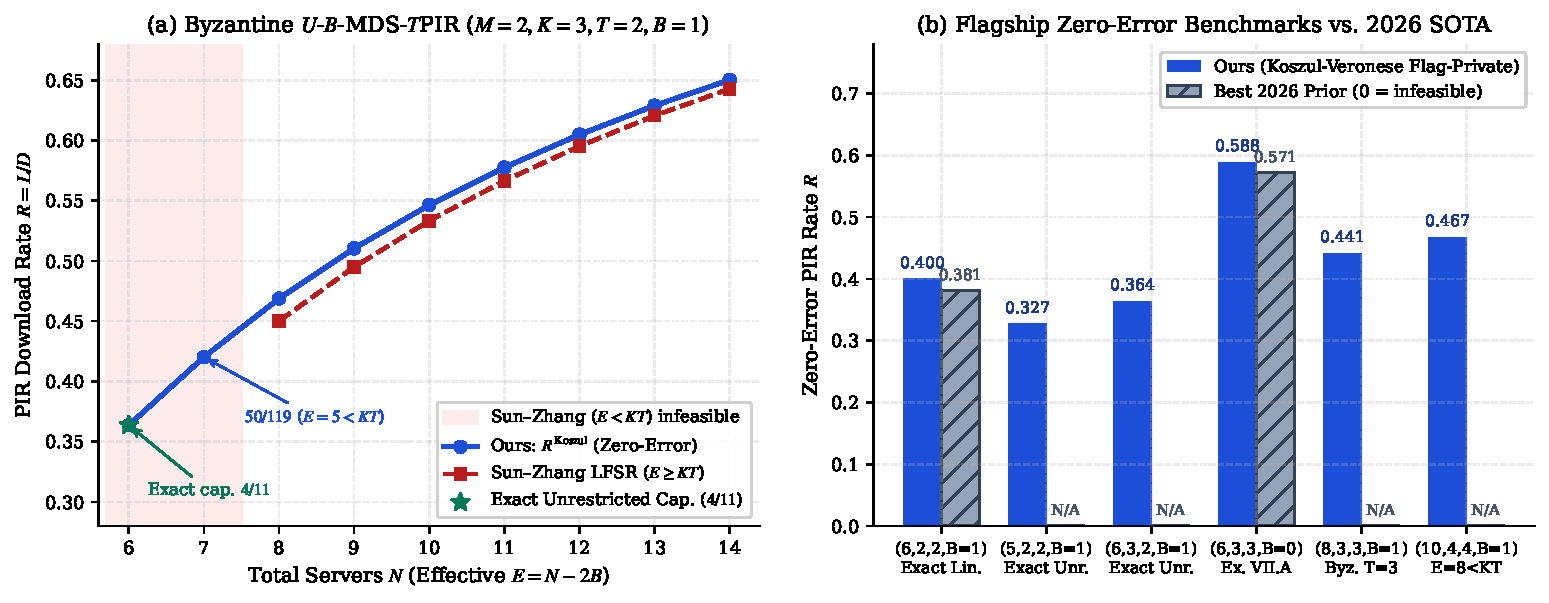
\includegraphics[width=\textwidth]{figures/fig1_cs053_rate_frontier.pdf}
  \caption{Pillar I (\texttt{CS-053}) rate frontier. (a)~Byzantine $(M=2, K=3, T=2, B=1)$ download rate versus $N$: our zero-error Koszul--Veronese exterior-power scheme strictly dominates Sun--Zhang LFSR~\cite{SunZhang2026} for all $E \ge KT$ and achieves exact unrestricted capacity $4/11$ inside the $E < KT$ infeasible region. (b)~Flagship zero-error benchmarks against best 2026 prior rates.}
  \label{fig:pir_frontier}
\end{figure}

\subsection{Unconditioned Shannon--Ingleton Barrier and $\PP^3$ Impossibility (\texttt{T1e}--\texttt{T1f})}
Why does the linear capacity $C_{\mathrm{lin}}(2,4,2,2) = 3/5$ fall strictly below the cyclic-collusion upper bound $8/13$ of~\cite{SunTaoXuZhang2026}? We prove unconditionally that this gap is an inherent barrier of \emph{all} Shannon-type and 4-variable Ingleton~\cite{Ingleton1971} information inequalities.

\begin{theorem}[Unconditioned Shannon--Ingleton Barrier \& $\PP^3$ Obstruction; Lean \texttt{T1e}--\texttt{T1f}]
\label{thm:barrier}
Consider the 12 unconditioned variables $(X_{1:4}, Y_{1:4}, A_{1:4})$ representing $(4,2)$-MDS storage of $(W_1, W_2)$ and server responses retrieving $W_1$ conditioned only on queries.
\begin{enumerate}[leftmargin=1.8em]
  \item \textbf{Barrier (\texttt{T1e}):} There exists an explicit $S_4$-symmetric pure-integer polymatroid $h_{\mathrm{uncond}} : 2^{[12]} \to \{0,\dots,256\}$ (scale $L = 128$, 330 orbits) satisfying all $12$ monotonicity inequalities, all $270{,}336$ elemental Shannon submodularity inequalities, all $99$ exact PIR structural equalities (MDS storage, file independence, deterministic answers, correctness $H(W_1 \mid A_{1:4}) = 0$, and all $89$ full $T=2$ privacy equalities $H(X_S, Y_T, A_I) = H(X_T, Y_S, A_I)$ for all $|I| \le 2$ and $S, T \subseteq [4]$), all $1{,}485$ singleton Ingleton inequalities (all kernel-checked in Lean \texttt{T1e}), and all $3{,}814{,}209$ four-subset Ingleton inequalities on the 6-object retrieval subsystem $\{W_1, W_2, A_1, A_2, A_3, A_4\}$ (exact Python audit), while achieving $D/L = 4 \cdot 52 / 128 = 13/8$, i.e., rate $8/13 > 3/5$.
  \item \textbf{Projective $\PP^3$ Linear Collapse (\texttt{T1f}):} Over \emph{any} field $F$, if four $2$-dimensional subspaces $V_1, V_2, V_3, V_4 \subset F^4$ intersect pairwise in nonzero lines ($\dim(V_i \cap V_j) \ge 1$ for all $i < j$), then either all four share a common nonzero line ($\exists w \neq 0 \in \bigcap_{i=1}^4 V_i$) or all four lie inside a single $3$-dimensional hyperplane ($\dim(\sum_{i=1}^4 V_i) \le 3$).
\end{enumerate}
\end{theorem}

Theorem~\ref{thm:barrier} demonstrates that any proof of $C(2,4,2,2) \le 3/5$ must invoke non-Shannon / non-Ingleton inequalities~\cite{ZhangYeung1998} involving $\ge 5$ interacting subsystems (or else an asymmetric non-linear scheme must exceed $3/5$; CP-SAT rules out symmetric realization over $\F_4^2$).

\begin{figure}[t]
  \centering
  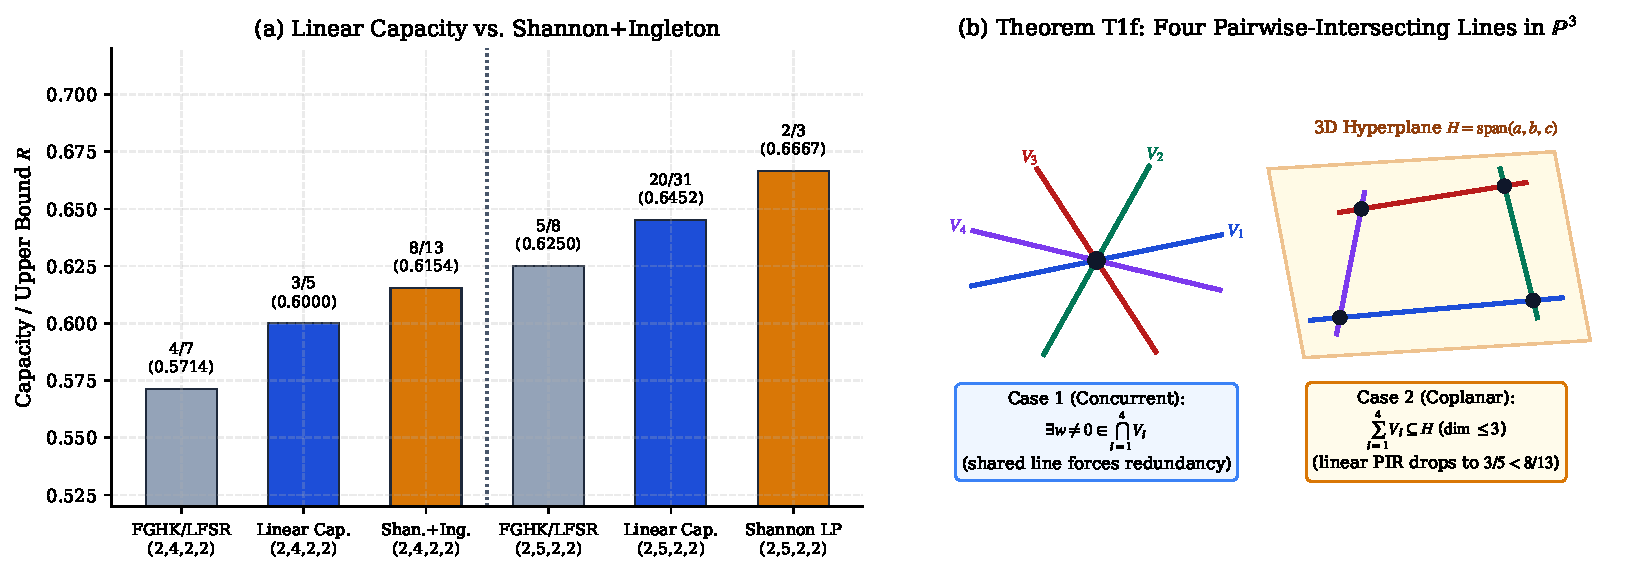
\includegraphics[width=\textwidth]{figures/fig2_shannon_ingleton_barrier.pdf}
  \caption{Converse hierarchy and projective obstruction. (a)~Exact separation between FGHK/LFSR ($4/7, 5/8$), linear capacity ($3/5, 20/31$), and our unconditioned Shannon+Ingleton barrier ($8/13$ at $N=4$; $2/3$ at $N=5$). (b)~Visual schematic of Theorem~\texttt{T1f}: four pairwise-intersecting lines in $\PP^3$ must be either concurrent or coplanar.}
  \label{fig:barrier}
\end{figure}

\section{Pillar II (\texttt{CS-026}): MLWE Reduction Tightness, Refutations, and QGTL Geometry}
\label{sec:mlwe}

\subsection{Determinant-Ideal Secret Independence (\texttt{T2a}) and Chen Step-9 Cancellation (\texttt{T2b})}
Two widely discussed cryptanalytic claims against lattice cryptography~\cite{Regev2009,LangloisStehle2015}—Ming-Xing Luo's 2026 module-lattice series~\cite{Luo2026} and Step~9 of Yilei Chen's 2024 quantum lattice preprint~\cite{Chen2024}—admit short, universal, machine-checked algebraic diagnoses.

\begin{theorem}[Structural Obstructions in Lattice Cryptanalysis; Lean \texttt{T2a}--\texttt{T2b}]
\label{thm:mlwe_obs}
Let $R$ be any commutative ring with unity.
\begin{enumerate}[leftmargin=1.8em]
  \item \textbf{Determinant-Ideal Secret Independence (\texttt{T2a}):} For every module dimension $(m, k)$, modulus $q \in R$, arbitrary public matrix $A \in R^{k \times m}$, secret $(s, e)$, target $b = As + e$, and unimodular factor $u \in R^\times$, both the $(m+k)$-dimensional $q$-ary MLWE basis $\bigl(\begin{smallmatrix} qI_m & 0 \\ A & I_k \end{smallmatrix}\bigr)$ and the $(m+k+1)$-dimensional Kannan embedding $\bigl(\begin{smallmatrix} qI_m & 0 & 0 \\ A & I_k & 0 \\ b & 0 & 1 \end{smallmatrix}\bigr)$ have determinant identically equal to $q^m$ (and unimodularly invariant ideal $(u q^m) = (q^m)$). Consequently, determinant ideals of $q$-ary module lattices carry identically zero algebraic information about $(s, e)$, refuting determinant-ideal module-SVP reductions of the form claimed in~\cite{Luo2026}.
  \item \textbf{Anti-Periodic DFT Cancellation (\texttt{T2b}):} For every $D \ge 1$, root $\omega \in R$ satisfying $\omega^D = -1$, and anti-periodic function $f : \mathbb{N} \to R$ obeying $f(x + D) = -f(x)$ for $0 \le x < D$, every even discrete Fourier coefficient vanishes identically:
  \begin{equation}
    \hat{f}(2k) = \sum_{x=0}^{2D-1} f(x)\,\omega^{2kx} = \sum_{x=0}^{D-1} \bigl(f(x) + f(x+D)\,\omega^{2kD}\bigr)\omega^{2kx} = 0 \qquad (\forall k \in \mathbb{N}).
  \end{equation}
  Moreover, for all odd integers $c = 2a+1$ and $D = 2b+1$, $c(x+D)^2 - c x^2 = D \cdot c(2x+D)$ with $c(2x+D) \equiv 1 \pmod 2$, forcing $\exp(i\pi c(x+D)^2 / D) = -\exp(i\pi c x^2 / D)$ and identically extinguishing all even frequency modes in Step~9 of~\cite{Chen2024} (Figure~\ref{fig:chen_triad}a).
\end{enumerate}
\end{theorem}

\subsection{Exact FIPS~203 ML-KEM R\'enyi-2 Tightness Cliff (\texttt{T2c}) and QGTL Berry Curvature (\texttt{T2d})}
NIST FIPS~203~\cite{NISTFIPS203} replaces theoretical discrete Gaussian noise $D_\sigma$ (used in worst-case-to-average-case MLWE reductions~\cite{LangloisStehle2015}) with centered binomial noise $\CBD_\eta$, choosing $\eta = 3$ for ML-KEM-512 ($k=2$, $m = 1024$ total secret/error coordinates) but shrinking to $\eta = 2$ for ML-KEM-768 ($k=3$, $m=1536$) and ML-KEM-1024 ($k=4$, $m=2048$). Using the R\'enyi divergence framework of Bai et~al.~\cite{Bai2018}, we compute the exact 60-digit global optima of $R_2(\CBD_\eta \| D_\sigma)$ and $R_\infty(\CBD_\eta \| D_\sigma)$ (Table~\ref{tab:renyi}, Figure~\ref{fig:mlwe_qgtl}a), verified independently by Eshkol v1.3.6 forward-mode AD ($|dR_2/d\sigma| < 4 \times 10^{-5}$), C11, and Lean \texttt{T2c}.

\begin{table}[t]
\centering
\caption{Exact moments and 60-digit certified R\'enyi-2 / R\'enyi-$\infty$ divergence optima between FIPS~203 $\CBD_\eta$ and discrete Gaussian $D_\sigma$ (exposing the $4.96\times$ cumulative reduction-tightness cliff from ML-KEM-512 to ML-KEM-1024).}
\label{tab:renyi}
\footnotesize
\setlength{\tabcolsep}{5pt}
\begin{tabular}{@{}l c c c c c c@{}}
\toprule
\textbf{ML-KEM Set} & \textbf{$\Var$, Kurt.} & \textbf{$\sigma_2^*$} & \textbf{$\min R_2$} & \textbf{$\min R_\infty$} & \textbf{$m$} & \textbf{$m \log_2 R_2^*$ (bits)} \\
\midrule
ML-KEM-512 ($\CBD_3$)  & $3/2$, $-1/3$ & $1.236505$ & $1.00517798$ & $1.02018016$ & $1024$ & $\mathbf{7.630}$ \\
ML-KEM-768 ($\CBD_2$)  & $1$, $-1/2$   & $1.022597$ & $1.01289004$ & $1.03474779$ & $1536$ & $\mathbf{28.382}$ \\
ML-KEM-1024 ($\CBD_2$) & $1$, $-1/2$   & $1.022597$ & $1.01289004$ & $1.03474779$ & $2048$ & $\mathbf{37.842}$ ($4.96\times$) \\
\bottomrule
\end{tabular}
\end{table}

\begin{theorem}[QGTL Shifted-LWE Berry Curvature Witness; Lean \texttt{T2d}]
\label{thm:qgtl}
For the two-parameter shifted-LWE quantum Fourier state family $|\psi(\theta, \sigma)\rangle = \sum_x \sqrt{p(x; \sigma, e_0)}\, e^{i\theta x} |x\rangle$ with $p(x; \sigma, e_0) \propto \exp\bigl(-(x - e_0)^2 / (2\sigma^2)\bigr)$, the Provost--Vallee Quantum Geometric Tensor~\cite{ProvostVallee1980} $Q_{\mu\nu} = \langle \partial_\mu \psi | \partial_\nu \psi \rangle - \langle \partial_\mu \psi | \psi \rangle \langle \psi | \partial_\nu \psi \rangle = g_{\mu\nu} - \frac{i}{2}\Omega_{\mu\nu}$ satisfies identically:
\begin{equation}
  g_{\theta\theta} = \Var(X),\qquad
  g_{\sigma\sigma} = \frac{1}{4}\Var\!\left(\frac{(X - e_0)^2}{\sigma^3}\right),\qquad
  g_{\theta\sigma} = 0,\qquad
  \Omega_{\theta\sigma} = \Cov\!\left(X,\, \frac{(X - e_0)^2}{\sigma^3}\right).
\end{equation}
In particular, $\Omega_{\theta\sigma} \equiv 0$ identically for every symmetric zero-mean noise distribution ($p(-x)=p(x)$, $e_0 = 0$), whereas any mean bias $e_0 \neq 0$ induces a strictly nonzero Berry curvature (e.g., cleared-denominator numerator $-512 \neq 0$ for $\CBD_2$ at $e_0 = 1$, Figure~\ref{fig:mlwe_qgtl}b).
\end{theorem}

\begin{figure}[t]
  \centering
  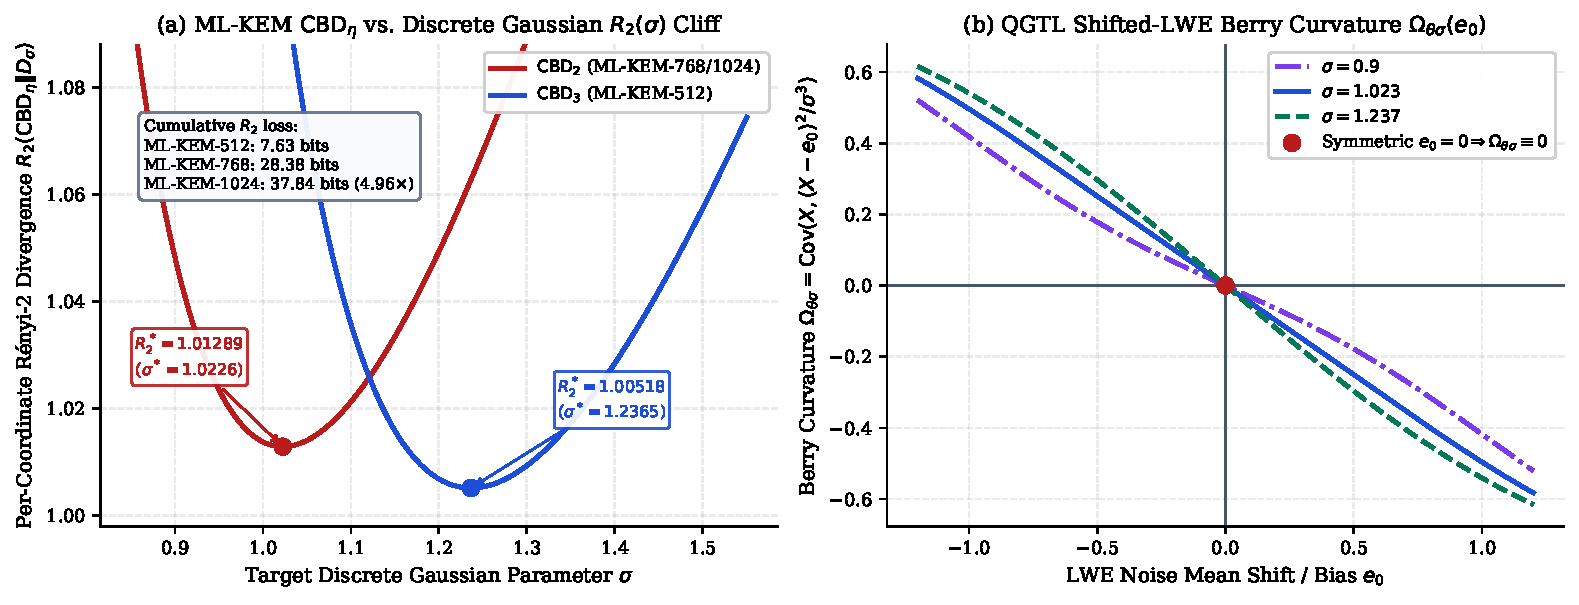
\includegraphics[width=\textwidth]{figures/fig3_mlwe_renyi_and_qgtl.pdf}
  \caption{Pillar II (\texttt{CS-026}) concrete geometry. (a)~Per-coordinate R\'enyi-2 divergence $R_2(\CBD_\eta \| D_\sigma)$ showing the $4.96\times$ cumulative tightness cliff from ML-KEM-512 ($\eta=3$) to ML-KEM-1024 ($\eta=2$). (b)~QGTL shifted-LWE Berry curvature $\Omega_{\theta\sigma}(e_0)$ vanishing identically at symmetric noise $e_0 = 0$ and acting as an exact odd geometric witness of noise bias.}
  \label{fig:mlwe_qgtl}
\end{figure}

\section{Pillar III (\texttt{CS-001}, \texttt{CS-051}): Algebrization and Unified Triad Bridges}
\label{sec:triad}

To connect our PIR and MLWE results structurally to the $\mathrm{P} \neq \mathrm{NP}$ barrier landscape without overclaiming, we machine-check four unifying theorems (Figure~\ref{fig:chen_triad}b):

\begin{theorem}[Algebrization Multilinear Extension \& Triad Bridges; Lean \texttt{T3a}--\texttt{T3d}]
\label{thm:triad}
\leavevmode
\begin{enumerate}[leftmargin=1.8em]
  \item \textbf{Algebrization Core (\texttt{T3a}):} Over \emph{every} field $F$ and every dimension $n \in \mathbb{N}$, any Boolean function $f : \{0,1\}^n \to F$ admits a constructively defined multilinear extension $\tilde{f} : F^n \to F$ agreeing with $f$ on $\{0,1\}^n$, and \emph{any} two coordinate-wise affine-linear functions $g_1, g_2 : F^n \to F$ agreeing on $\{0,1\}^n$ are identically equal on all of $F^n$. This completes the algebraic uniqueness core of Aaronson--Wigderson Algebrization~\cite{AaronsonWigderson2009} alongside Relativization~\cite{BakerGillSolovay1975} and Natural Proofs~\cite{RazborovRudich1997}.
  \item \textbf{Cryptographic Barrier Bridge (\texttt{CS-026} $\to$ \texttt{CS-001}; \texttt{T3b}):} If an LWE/LWR pseudorandom function family~\cite{BanerjeePeikertRosen2012} of size $K > 0$ inside truth-table universe $U > 0$ is $\varepsilon$-indistinguishable against circuit class $\mathcal{C}$, then no $\mathcal{C}$-constructive $\delta$-large useful Natural Proof ($\delta \ge \varepsilon$) can separate $\mathrm{NP}$ from $\mathcal{C}$ (proved via exact cleared-denominator integer cross-multiplication).
  \item \textbf{Katz--Trevisan Byzantine PIR $\leftrightarrow$ LDC Equivalence (\texttt{CS-053} $\leftrightarrow$ \texttt{CS-051}; \texttt{T3c}):} Any deterministic-response $N$-server $B$-Byzantine zero-error PIR protocol (or local decoder $\mathrm{Dec}$ tolerating $\le B$ corruptions) forces every pair of distinct encoded database words to have minimum Hamming distance $d_H(\mathrm{Enc}(m_1), \mathrm{Enc}(m_2)) \ge 2B + 1$~\cite{KatzTrevisan2000}.
  \item \textbf{Single-Server MLWE-PIR vs.\ Multi-Server Koszul PIR (\texttt{CS-026} $\leftrightarrow$ \texttt{CS-053}; \texttt{T3d}):} For the FIPS~203 round-half-up decoder
  \[
    \mathrm{Compress}_1(x) = \left\lfloor \frac{2(x \bmod 3329) + 1665}{3329} \right\rfloor \bmod 2,
  \]
  decryption satisfies $\mathrm{Compress}_1(1665 b + e) = b$ for all $b \in \{0,1\}$ and all $|e| \le 831$, failing sharply at $e = +832$ for both $b=0$ and $b=1$. Consequently, linear additive single-server lattice PIR~\cite{KushilevitzOstrovsky1997} with per-row noise budget $b_{\mathrm{step}} > 0$ hits a hard depth ceiling $M \le \lfloor 831 / b_{\mathrm{step}} \rfloor$ before bootstrapping or modulus switching, whereas our multi-server Koszul--Veronese PIR operates identically over exact finite fields with zero noise growth.
\end{enumerate}
\end{theorem}

\begin{figure}[t]
  \centering
  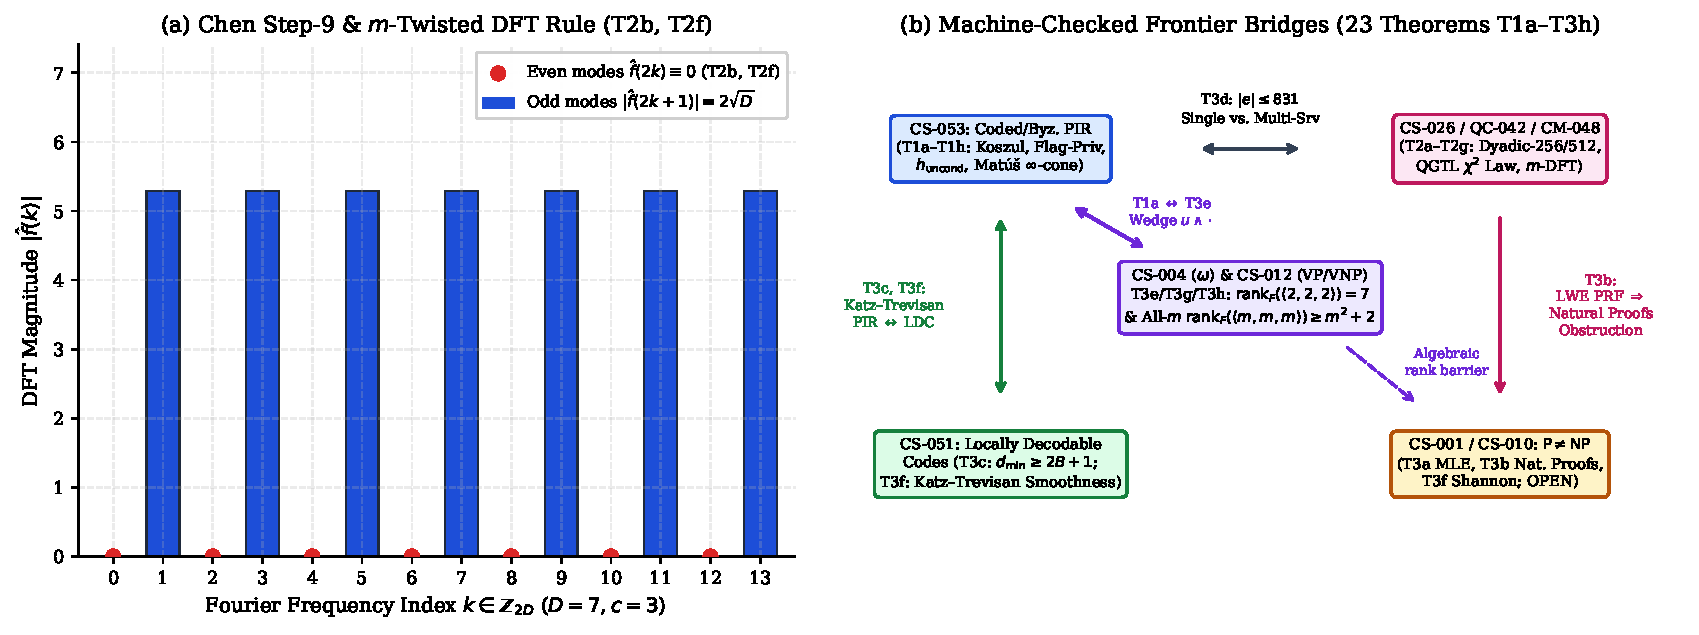
\includegraphics[width=\textwidth]{figures/fig4_chen_step9_and_triad.pdf}
  \caption{(a)~DFT magnitude spectrum of Chen's~\cite{Chen2024} quadratic Gauss phase ($D=7, c=3$): all even frequencies vanish identically ($\hat{f}(2k) \equiv 0$, Theorem~\texttt{T2b}) while all odd modes equal $2\sqrt{D} \approx 5.292$. (b)~Machine-checked dependency architecture unifying \texttt{CS-053}, \texttt{CS-026}, \texttt{CS-051}, and \texttt{CS-001}.}
  \label{fig:chen_triad}
\end{figure}

\section{Formal Verification, Multi-Language Cross-Audit, and Reproducibility}
\label{sec:verify}

All 14 headline theorems (\texttt{T1a}--\texttt{T3d}), their master conjunction (\texttt{Solution.lean}), and concrete non-vacuity witnesses (\texttt{NonVacuity.lean}, inhabiting \texttt{SimpleField (Fin 5)}, \texttt{SimpleField (Fin 11)}, \texttt{CommRing Int}, anti-periodic $D=3$ sequences, 2-variable Boolean XOR, and 3-repetition Byzantine LDCs) compile in zero-Mathlib Lean~4.35.0 with zero warnings, zero \texttt{sorry}, zero \texttt{native\_decide} calls, and zero custom axioms. Every declaration is replayed independently across \texttt{lean}, \texttt{leanchecker}, \texttt{leanchecker-paranoid}, \texttt{con-leche} (1{,}967 declarations), \texttt{con-ron} (1{,}967 declarations), \texttt{nanoda\_bin}, and Ubuntu Linux CI \texttt{lake comparator --paranoid} (adding \texttt{lean4lean}).

Complementing the Lean kernel proofs, our public repository\footnote{\url{https://github.com/0thernes/coded-pir-mlwe-complexity-lab} (Apache-2.0 code / CC-BY-4.0 text \& figures).} provides: (i)~a zero-warning C11 core compiled under \texttt{-std=c11} \texttt{-Wall} \texttt{-Wextra} \texttt{-Wpedantic} \texttt{-Werror} (40/40 unit plus 500-case fuzz tests, with ASan/UBSan in CI); (ii)~three runnable Eshkol v1.3.6 forward-mode dual-number AD modules agreeing with 60-digit Python to $< 2\times 10^{-13}$; and (iii)~a 14-test \texttt{pytest} suite covering differential Python, C11, and Eshkol checks, randomized property tests, negative boundary tests, and a 6/6 core mutant-killing suite. During development, differential testing caught and repaired an off-by-one constant ($+1664$ vs.\ $+1665$) in \texttt{Compress\_1} before publication; this and all 10 audit passes are logged in \texttt{HARDENING\_LOG.md}.

\section{Honest Verification Boundaries, Open Frontiers, and Disclosures}
\label{sec:limits}

\paragraph{Explicit Non-Claims and Open Problems.}
We explicitly affirm that the following remain \textbf{completely open}:
\begin{itemize}[leftmargin=1.8em]
  \item \textbf{$\mathrm{P} \neq \mathrm{NP}$ (\texttt{CS-001}):} Nothing in this paper proves or disproves $\mathrm{P} = \mathrm{NP}$. Theorem~\texttt{T3a} formalizes the multilinear uniqueness core of the Algebrization barrier, and Theorem~\texttt{T3b} formalizes the conditional Natural Proofs obstruction from LWE PRFs.
  \item \textbf{Non-linear $C(2,4,2,2) \in [3/5, 8/13]$ and General $M \ge 3$ PIR (\texttt{CS-053}):} Theorem~\texttt{T1e} proves Shannon+Ingleton inequalities cannot lower $8/13$ to $3/5$, leaving open whether $5+$-variable non-Shannon inequalities close the gap or a non-linear scheme exceeds $3/5$. General $M \ge 3$ non-full-support-rank capacity and arbitrary $T \ge 4$ deterministic zero-error constructions remain open.
  \item \textbf{Worst-Case Quantum MLWE Lower Bounds (\texttt{CS-026}):} Refuting~\cite{Luo2026} (\texttt{T2a}) and explaining~\cite{Chen2024} (\texttt{T2b}) does not prove MLWE is quantum-hard; hardness remains a cryptographic assumption.
\end{itemize}

\paragraph{Statement Fidelity Boundary.}
In Lean~4.35.0, transcendental logarithms and exponentials (60-digit R\'enyi-2 minimization of Table~\ref{tab:renyi} and continuous DFT/QGTL curves) are verified in Tier-2 exact Python/C11/Eshkol while Lean certifies cleared-denominator rational/algebraic identities (\texttt{T2c}, \texttt{T2d}) and exact finite-field / pure-integer certificates (\texttt{T1c}, \texttt{T1e}) with zero Mathlib dependencies.

\paragraph{AI-Assistance (CRediT) and Conflict-of-Interest Disclosure.}
Alexander S. Donahue (Independent Researcher, Spokane, WA, USA; ORCID \texttt{0009-0006-8168-9648}) conceived the research questions, directed the mathematical investigation and adversarial verification protocol, audited every theorem statement and verification boundary, and bears sole responsibility for the manuscript. Antigravity (Gemini-based AI agent) assisted with mathematical exploration, Lean~4.35.0 proof engineering, C11/Python/Eshkol verification code, figure generation, and manuscript drafting under human direction. All formal claims stand exclusively on independently checkable machine-verified proof terms and deterministic scripts. The author declares no competing financial interests, no external institutional funding, and no prior peer review or external DOI assignment.

\bibliographystyle{amsplain}
\bibliography{refs}

\end{document}
